\subsection{\mu Master Module (\mu M)}

\mu M is a microcontroller that runs software to acquire, accumulate and request transmission of water flow measurements.

\subsubsection{Requirements}
Almost any microcontroller is able to accomplish this task.
Physical space is not critical, therefore we use a readily available low cost  Arduino Development Kit (DK)
DK, rather than designing a custom board. Given the absence of more specific requirements,
I choose the \cite{noauthor_arduino_2016-1} .

\subsubsection{Implementation}


\begin{table}[H]
    \centering
    \begin{tabularx}{\linewidth}{>{\hsize=0.25\hsize}X
            >{\hsize=1\hsize}X >{\hsize=1\hsize}X
            >{\hsize=0.5\hsize}X >{\hsize=2.25\hsize}X}
        Id    & BOM Item                       & Order Code & Package  & Rationale                 \\
        \midrule
        $U_1$ & \cite{noauthor_arduino_2016-1} &            & DIL (28) & availability, ease of use \\
    \end{tabularx}
    \caption{\mu M - BOM}

\end{table}
\begin{table}[H]
    \centering
    \begin{threeparttable}[b]
        \begin{tabularx}{\linewidth}{ >{\hsize=.15\hsize}X >{\hsize=1.35\hsize}X >{\hsize=1.5\hsize}X }
            Id & Issue                                                 & Potential solutions                                             \\
            \midrule
            1  & $U_1$ has relatively high power consumption.\tnote{1} & low power \mu C (MSP430FR2311IPW16) and custom charger circuit. \\
            2  & $U_1$ requires a stable 5 V power supply.\tnote{2}    & see issue 1                                                     \\
        \end{tabularx}
        \begin{tablenotes}
            \item [1]   This is due to the microcontroller itself (SAM D21) and to the peripheral components (battery charger).
            \item [2]   Given that a \SI{3.7}{\V} LiPo battery is used, this requires a boost conversion which in turn implies losses.
        \end{tablenotes}
    \end{threeparttable}
    \caption{\mu M - Issues}

\end{table}
\clearpage
\begin{figure}[h]
    \centering
    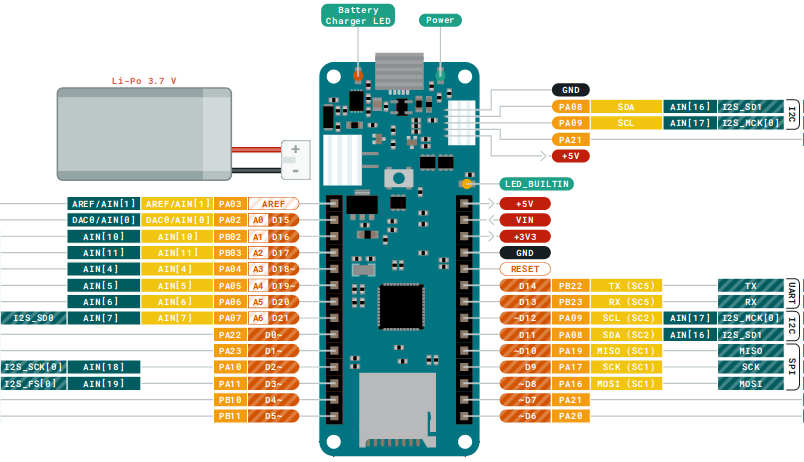
\includegraphics[width=0.9\textwidth]{MA/uM/uM}
    \caption{\mu M - pin out \cite{noauthor_arduino_2016-1}}
\end{figure}
\begin{table}[H]
    \centering
    \begin{threeparttable}[b]
        \begin{tabularx}{\linewidth}{ >
                    {\hsize=.25\hsize}X >
                    {\hsize=0.5\hsize}X >
                    {\hsize=.25\hsize}X  >
                    {\hsize=.5\hsize}X >
                    {\hsize=.25\hsize}X  >
                    {\hsize=3\hsize}X
            }
                  & \multicolumn{4}{c}{Pin mapping} &                                                                                                                   \\
            \cmidrule(lr){3-6}
            Id    & Net                             & Nb. & Name           & Type                           & Function                                                  \\
            \midrule
            $U_1$ & .Prx                            & 2   & \texttt{A0}    & \leftsquigarrow                & A/D conversion of OS output voltage                       \\
            $U_1$ & ESS                             & 9   & \texttt{D0}    & \rightharpoonup                & enable SS                                                 \\
            $U_1$ & ACK'                            & 10  & \texttt{D1}    & \leftharpoonup                 & .ACK connected via BI\textsubscript{1}                    \\
            $U_1$ & EOD                             & 11  & \texttt{D2}    & \rightharpoonup                & enable OD                                                 \\
            $U_1$ & EWD                             & 12  & \texttt{D3}    & \rightharpoonup                & enable WD                                                 \\
            $U_1$ & RWD                             & 13  & \texttt{D4}    & \rightharpoonup                & reset WD timer                                            \\
            $U_1$ & \neg .PB\tsc{1}                 & 14  & \texttt{D5}    & \leftharpoonup \upharpoonright & user push button                                          \\
            $U_1$ & .B'                             & 16  & \texttt{A1}    & \leftsquigarrow                & A/D conversion of scaled down battery voltage ( < 3.3 V)  \\
            $U_1$ & .S\textsubscript{1'c}           & 17  & \texttt{A2}    & \leftsquigarrow                & A/D conversion of scaled down solar voltage ( < 3.3 V)    \\
            $U_1$ & .S\textsubscript{2'c}           & 18  & \texttt{A3}    & \leftsquigarrow                & A/D conversion of scaled down solar voltage ( < 3.3 V)    \\
            $U_1$ & .SDA                            & 20  & \texttt{SDA}   & \leftrightharpoons             & .SDA connected via BI\textsubscript{2}                    \\
            $U_1$ & .SCL                            & 21  & \texttt{SCL}   & \leftrightharpoons             & .SCL connected via BI\textsubscript{2}                    \\
            $U_1$ & \neg RS                         & 24  & \texttt{RESET} & \leftharpoonup                 & pulled down by WD timer or user button in case of timeout \\
            $U_1$ & \Gnd                            & 25  & \texttt{GND}   & \Gnd                           &                                                           \\
            $U_1$ & 3V3                             & 26  & \texttt{VCC}   & $\rightarrow$                  & regulated output voltage\tnote{1}                         \\
            $U_1$ & .V\textsubscript{\mu M}         & 27  & \texttt{VIN}   & $\leftarrow$                   & unregulated input voltage >  \SI{3.5}{\V} \tnote{2}       \\
        \end{tabularx}
        \begin{tablenotes}
            \item [1] \begin{displayquote}[]\textelp{} This pin outputs 3.3V through the on-board voltage regulator.
                This voltage is the same regardless the power source
                used (USB, Vin and Battery) (\cite{noauthor_arduino_2016-1}).\end{displayquote}
            \item [2]  \begin{displayquote}[]\textelp{} This pin can be used to power the board with a regulated 5V source.
                If the power is fed through this pin, the USB power source is disconnected.
                This is the only way you can supply \SI{5}{V} (range is 5V to maximum 6V) to the board not using USB.
                (\cite{noauthor_arduino_2016-1}).             \end{displayquote}
        \end{tablenotes}
    \end{threeparttable}
\end{table}
\clearpage


